The L1L2 data set requires one track to have passed through the active region of Layer 1 with a corresponding hit and the other track to have a first hit in Layer 2. To ensure that a track did not miss Layer 1 due to an inefficiency, the Layer 2 track is extrapolated to Layer 1 and verified that it did not pass through the active region of the silicon sensor. The mass and $z$ vertex distribution for the L1L2 data taken with the SVT at 0.5~mm is shown in Figure~\ref{fig:zvm_l1l2}.
\begin{figure}[hbt]
\begin{minipage}{0.5\textwidth}
 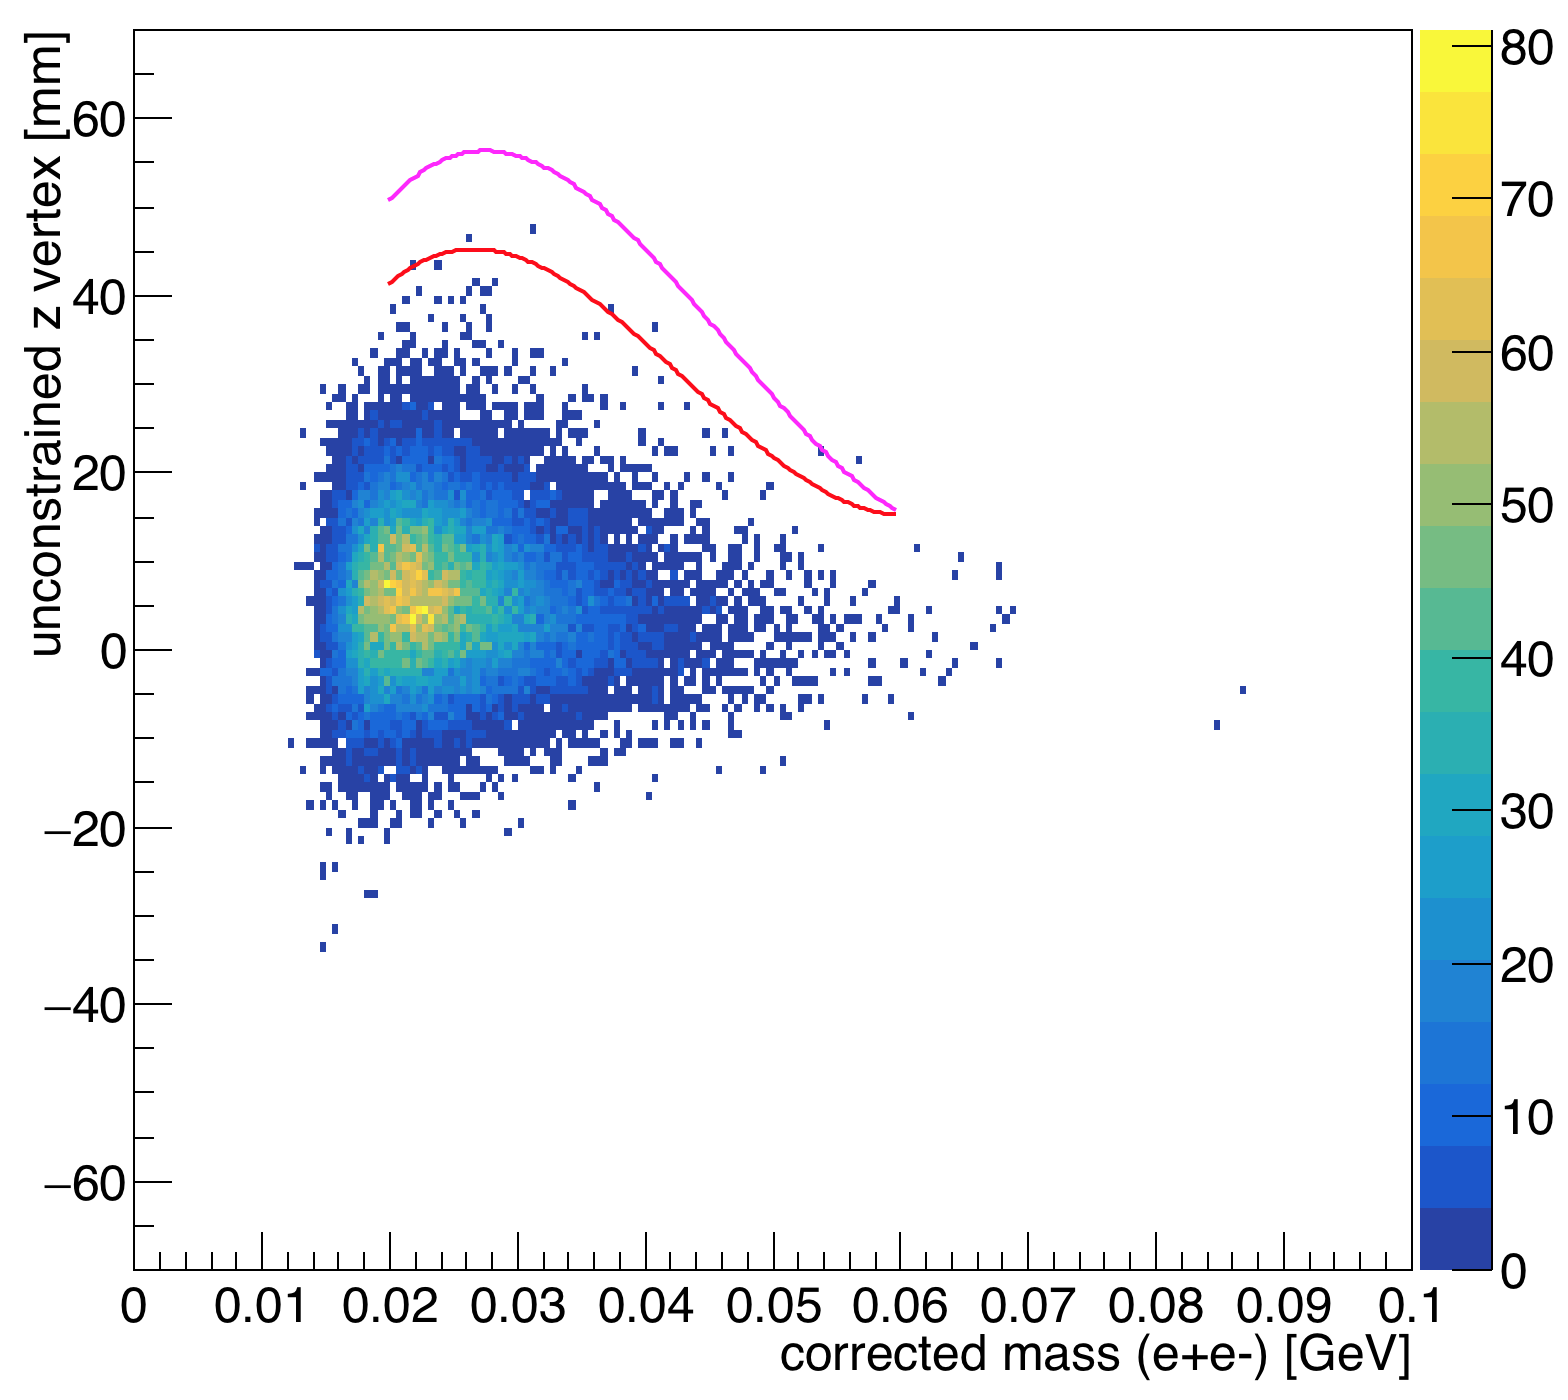
\includegraphics[width=\textwidth]{pics/appendix/zVm_L1L2_0p5_bl.png}
\end{minipage}\hfill\begin{minipage}{0.5\textwidth}
 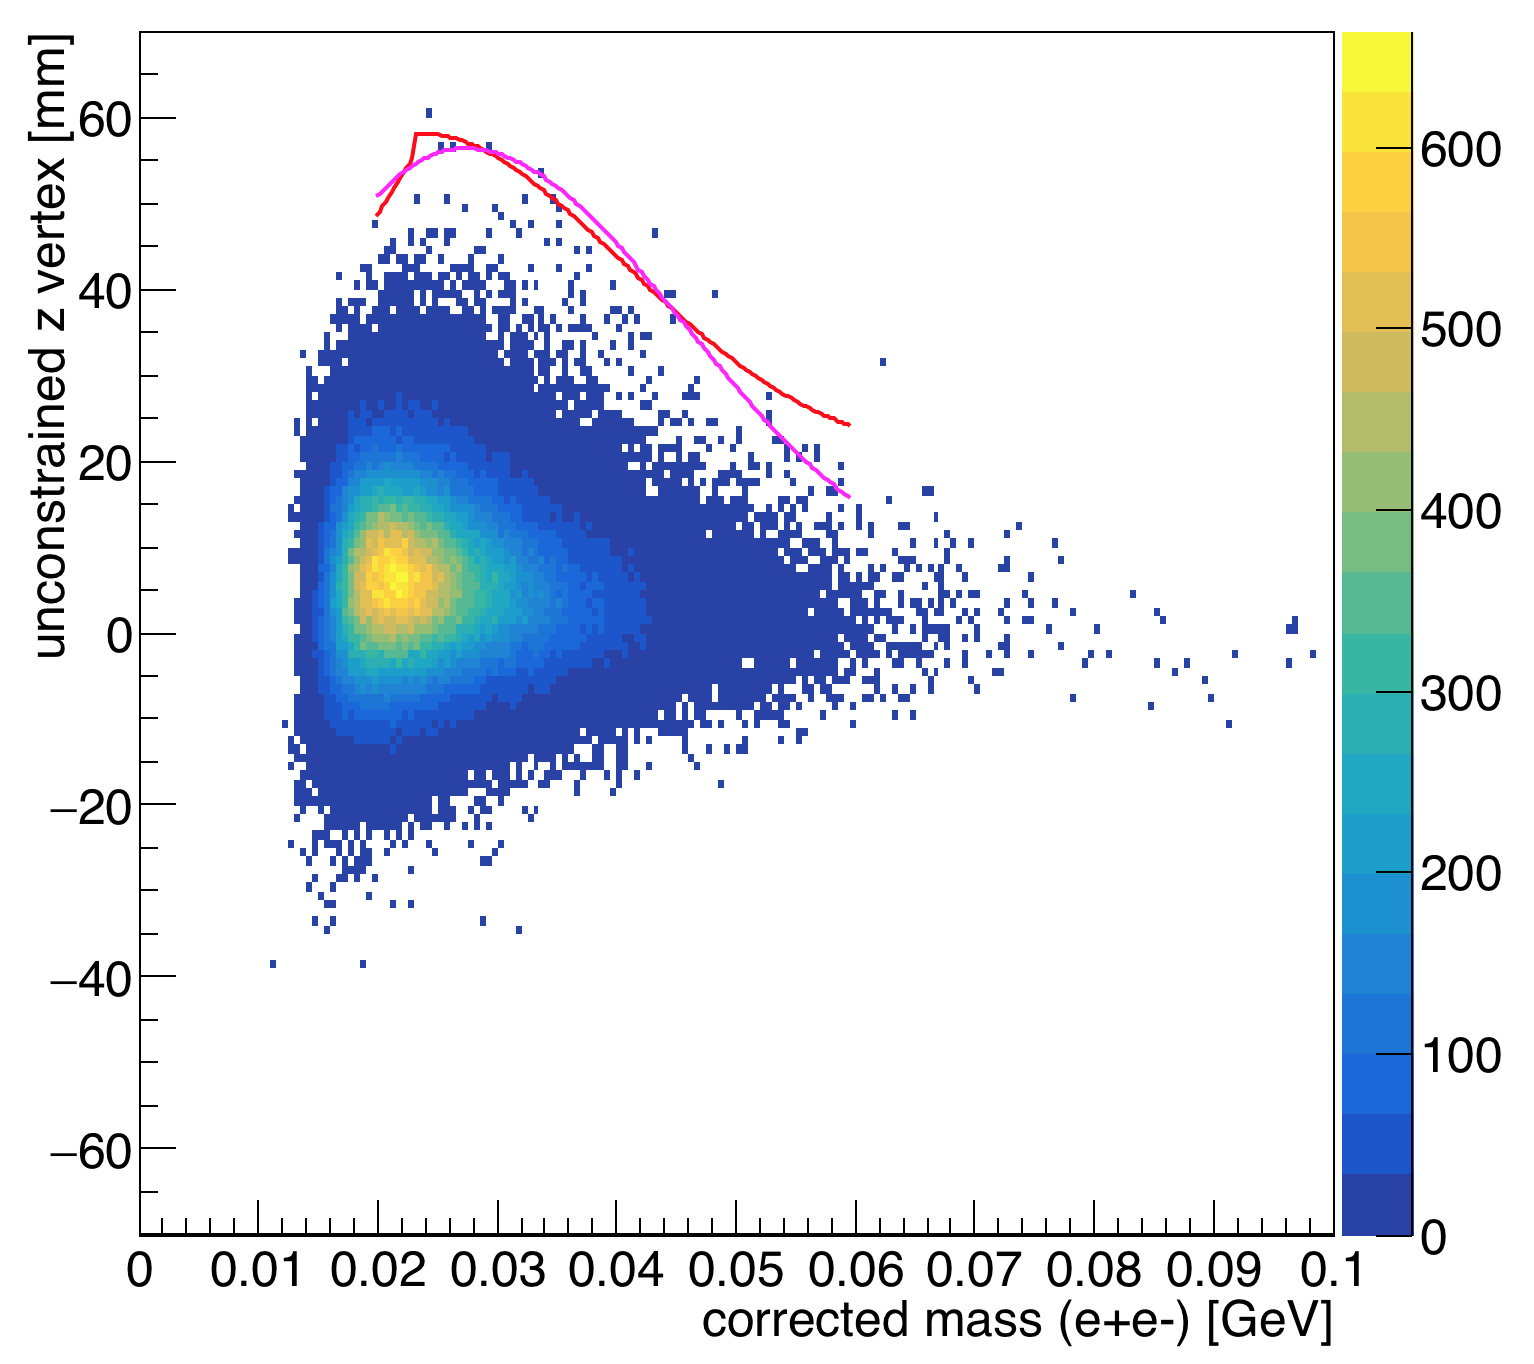
\includegraphics[width=\textwidth]{pics/appendix/zVm_L1L2_0p5_ub.png}
 \end{minipage}
  \caption[$z$ vertex and mass distribution for the L1L2 data set with the SVT at $\pm0.5$~mm]{The unconstrained $z$ vertex position is shown as a function of the corrected mass
of the $e^+e^-$ pair where one track has a hit in Layer 1 and the other track does not pass through the active region of Layer 1. The $zCut$ as measured for this data is shown in red
and corresponds to the full 100$\%$ data set where there is less than 0.5 background event beyond. The projected $zCut$ from the 10$\%$ of the data is shown in magenta. The relevant mass range used to measure $zCut$ is from 0.02--0.06~GeV based on measured statistics. The 10$\%$ sample for tuning cuts is shown on the left, and the full 100$\%$ of the data is shown on the right.}
  \label{fig:zvm_l1l2}
\end{figure}
The L1L2 data forces the $zCut$ to be very high due to the presence of a large high $z$ background component. WAB conversions in Layer 1 generally have an electron in Layer 1 and the positron track in Layer 2 (missing Layer 1). This accounts for most of the statistics of this data. However, even if the data is divided for events where the electron has a hit in Layer 1 and the positron has a hit in Layer 1, there are still large high $z$ backgrounds for each set. No one vertex cut (such as on the beam spot constraint quality) is able to remove these events. The measured $zCut$ for this data set is so large that the data cannot contribute to the reach. A significantly lower $zCut$ could restore some of the reach from this set, but the reach obtained is still much less than L1L1 data set. \\
\indent The mass and $z$ vertex distribution for the L1L2 data taken with the SVT at 1.5~mm is shown in Figure~\ref{fig:zvm_l1l2_1p5}.
\begin{figure}[hbt]
\begin{minipage}{0.5\textwidth}
 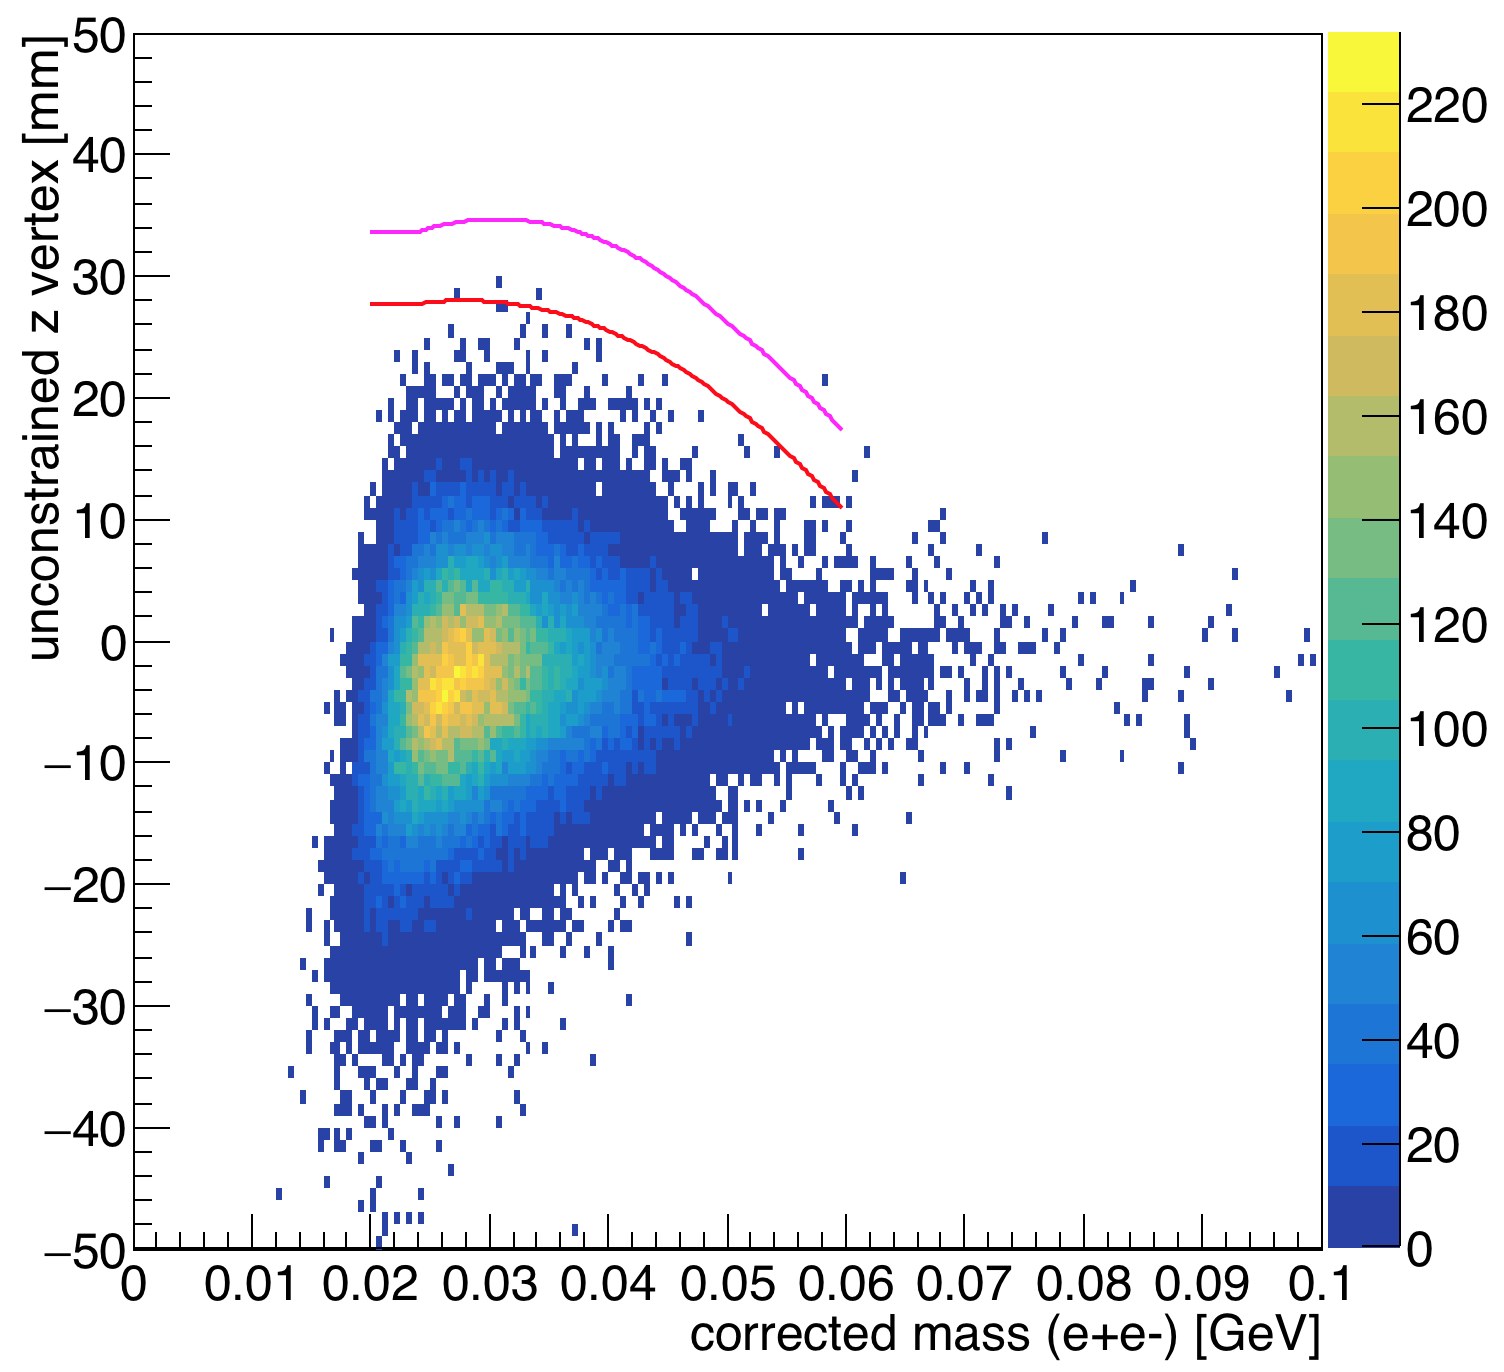
\includegraphics[width=\textwidth]{pics/appendix/zVm_L1L2_1p5_bl.png}
\end{minipage}\hfill\begin{minipage}{0.5\textwidth}
 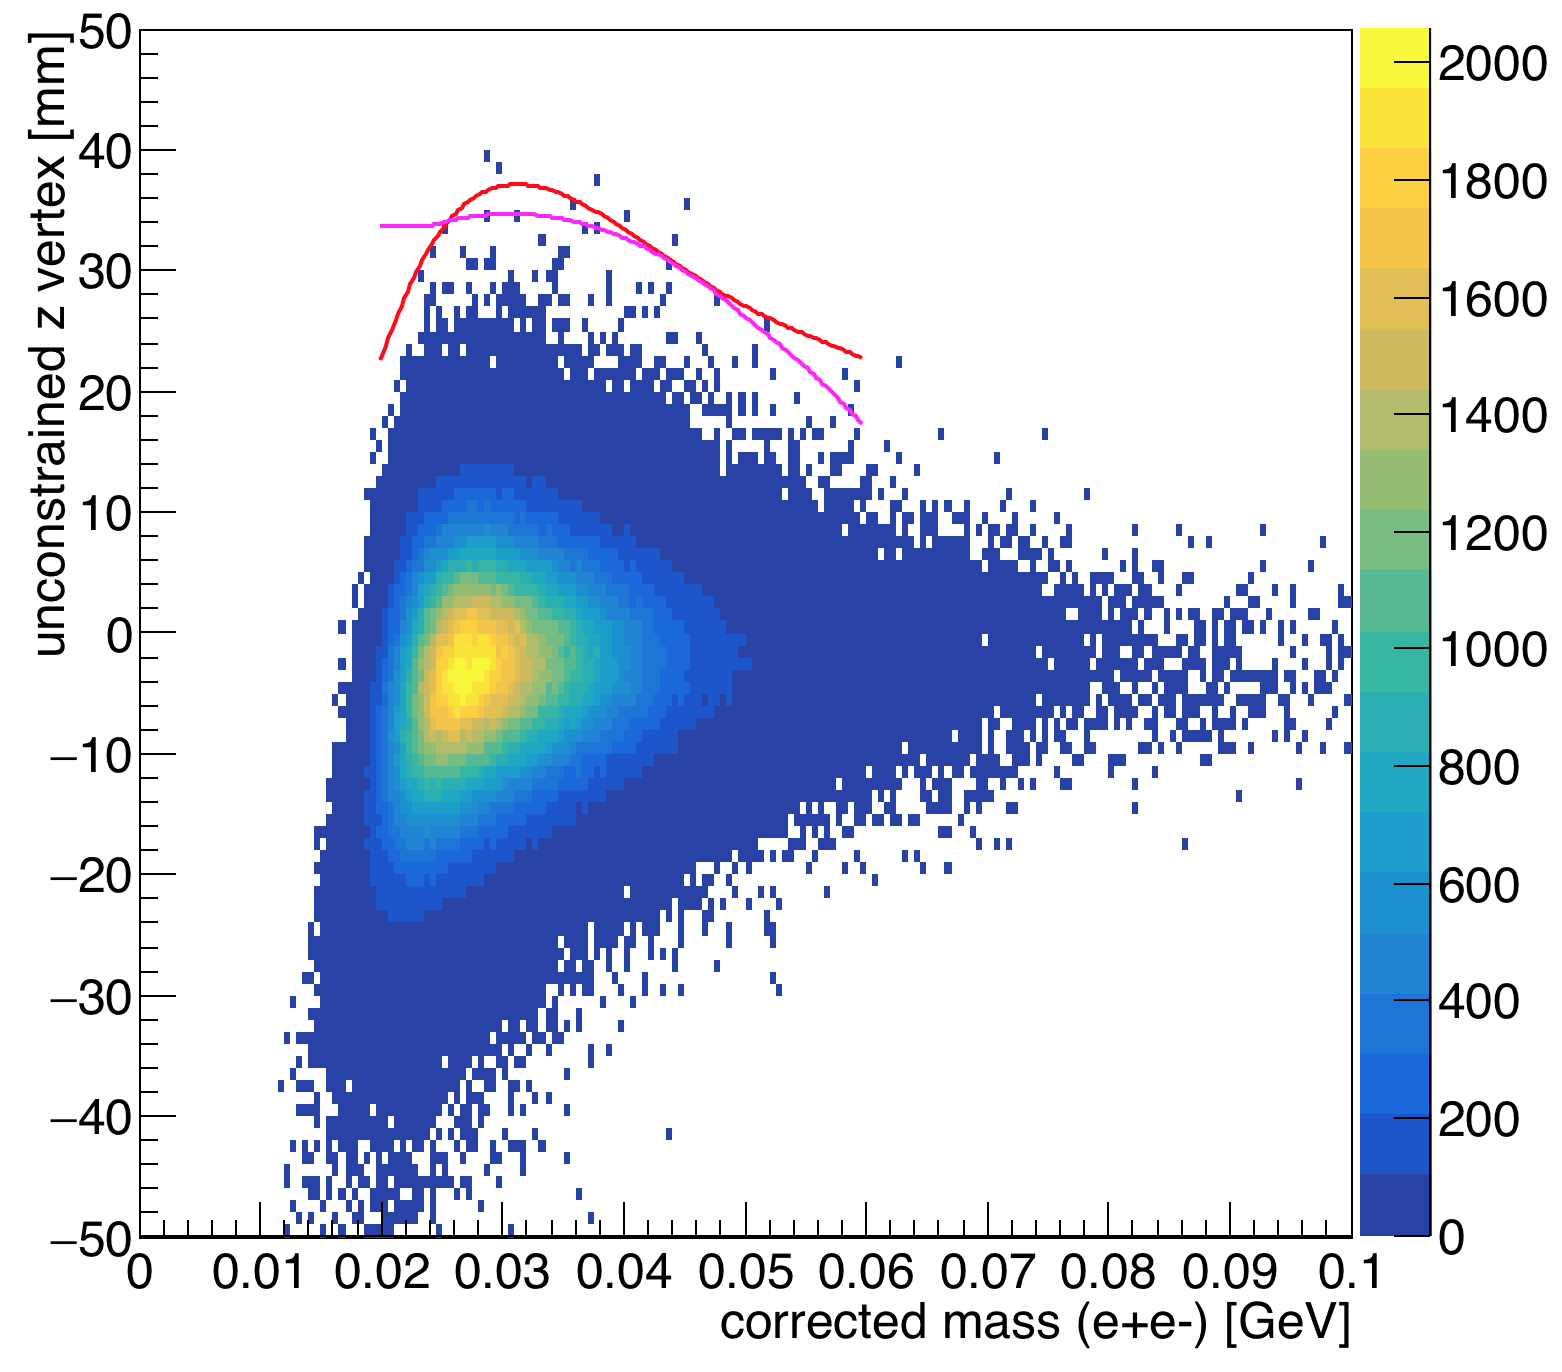
\includegraphics[width=\textwidth]{pics/appendix/zVm_L1L2_1p5_ub.png}
 \end{minipage}
  \caption[$z$ vertex and mass distribution for the L1L2 data set with the SVT at $\pm1.5$~mm]{The unconstrained $z$ vertex position is shown as a function of the corrected mass
of the $e^+e^-$ pair where one track has a hit in Layer 1 and the other track does not pass through the active region of Layer 1. The $zCut$ as measured for this data is shown in red
and corresponds to the full 100$\%$ data set where there is less than 0.5 background event beyond. The projected $zCut$ from the 10$\%$ of the data is shown in magenta. The relevant mass range used to measure $zCut$ is from 0.02--0.06~GeV based on measured statistics. The 10$\%$ sample for tuning cuts is shown on the left, and the full 100$\%$ of the data is shown on the right.}
  \label{fig:zvm_l1l2_1p5}
\end{figure}
This data has significantly fewer high $z$ background events than that shown in Figure~\ref{fig:zvm_l1l2}.\\
\indent The L2L2 data sets are composed of vertexed pairs of tracks that missed Layer 1 and extrapolate to the outside of the active region of the silicon sensor in Layer 1. The mass and $z$ vertex distribution for the L2L2 data taken with the SVT at 0.5~mm is shown in Figure~\ref{fig:zvm_l2l2}.
\begin{figure}[hbt]
\begin{minipage}{0.5\textwidth}
 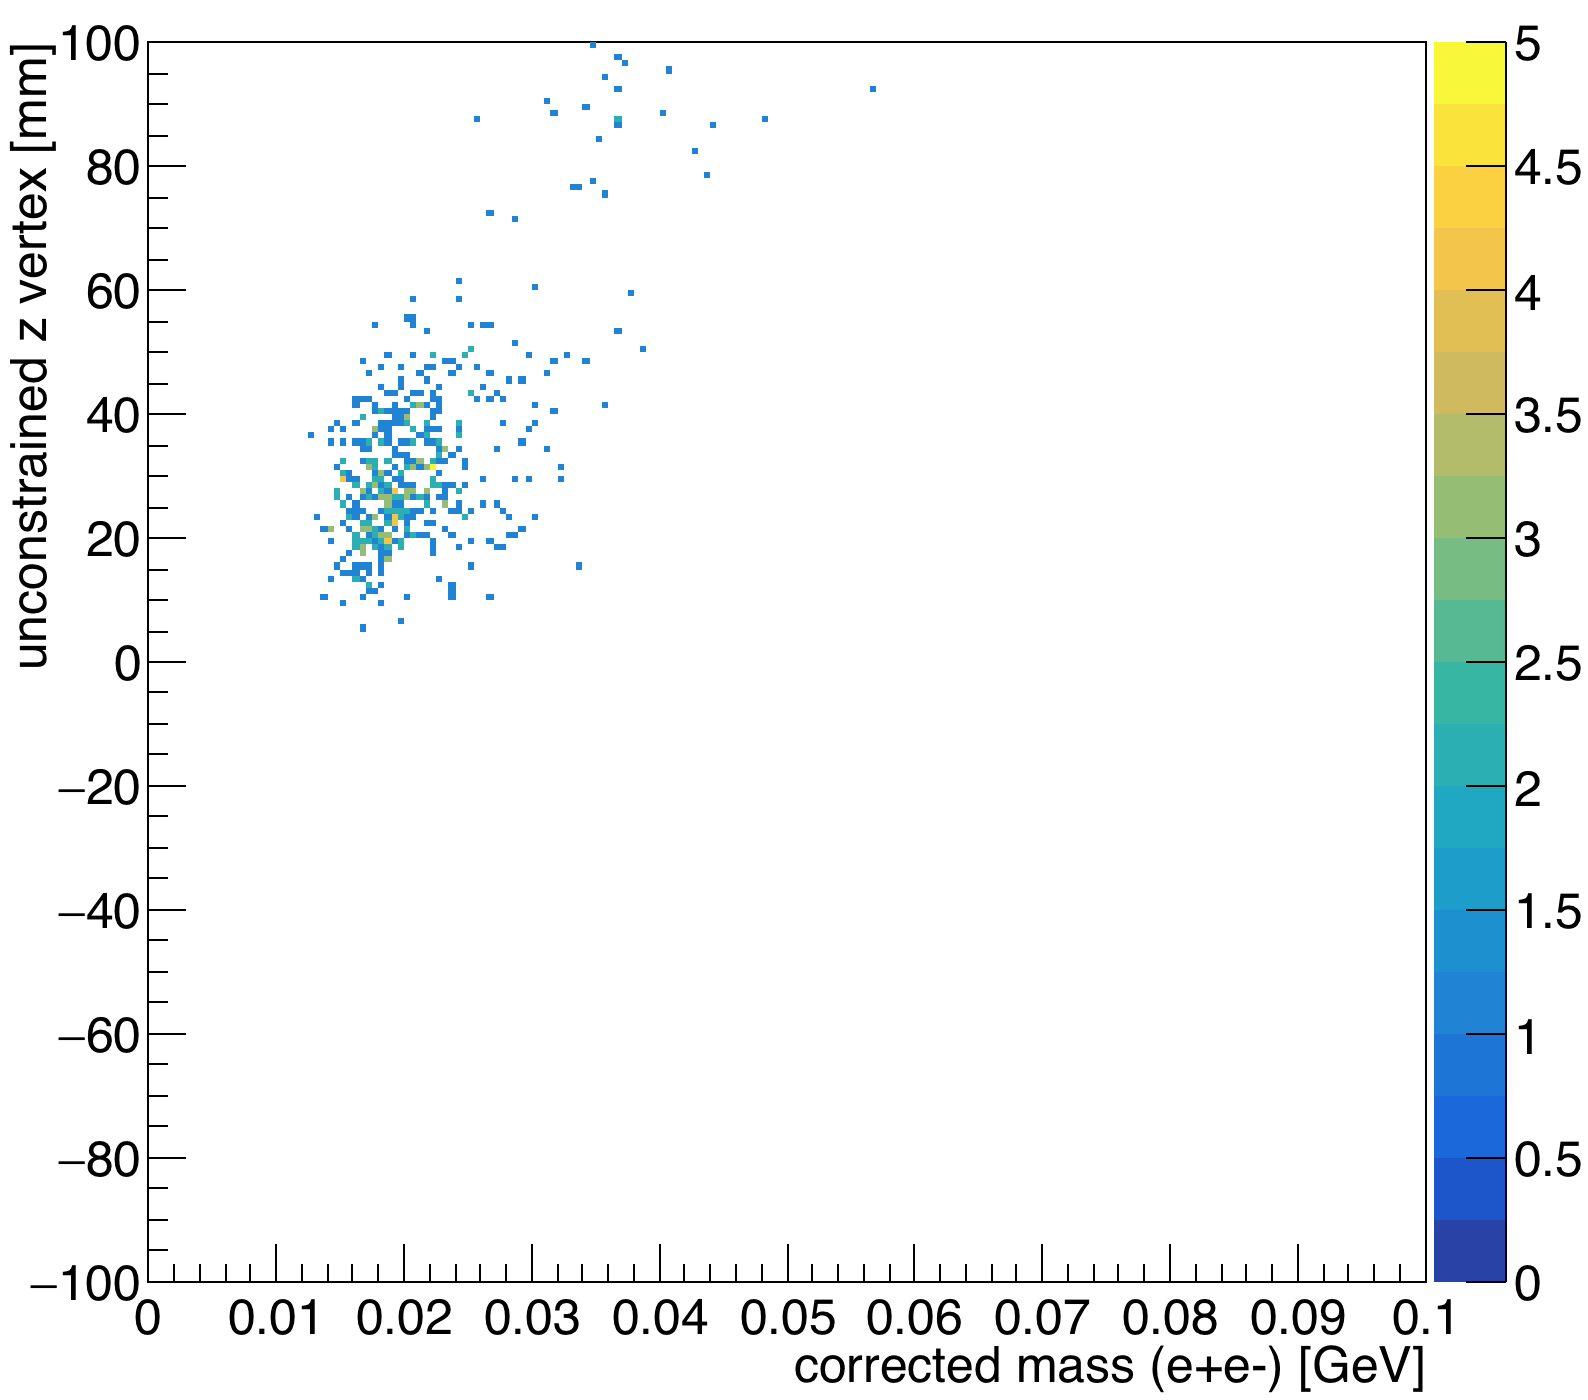
\includegraphics[width=\textwidth]{pics/appendix/zVm_L2L2_0p5_bl.png}
\end{minipage}\hfill\begin{minipage}{0.5\textwidth}
 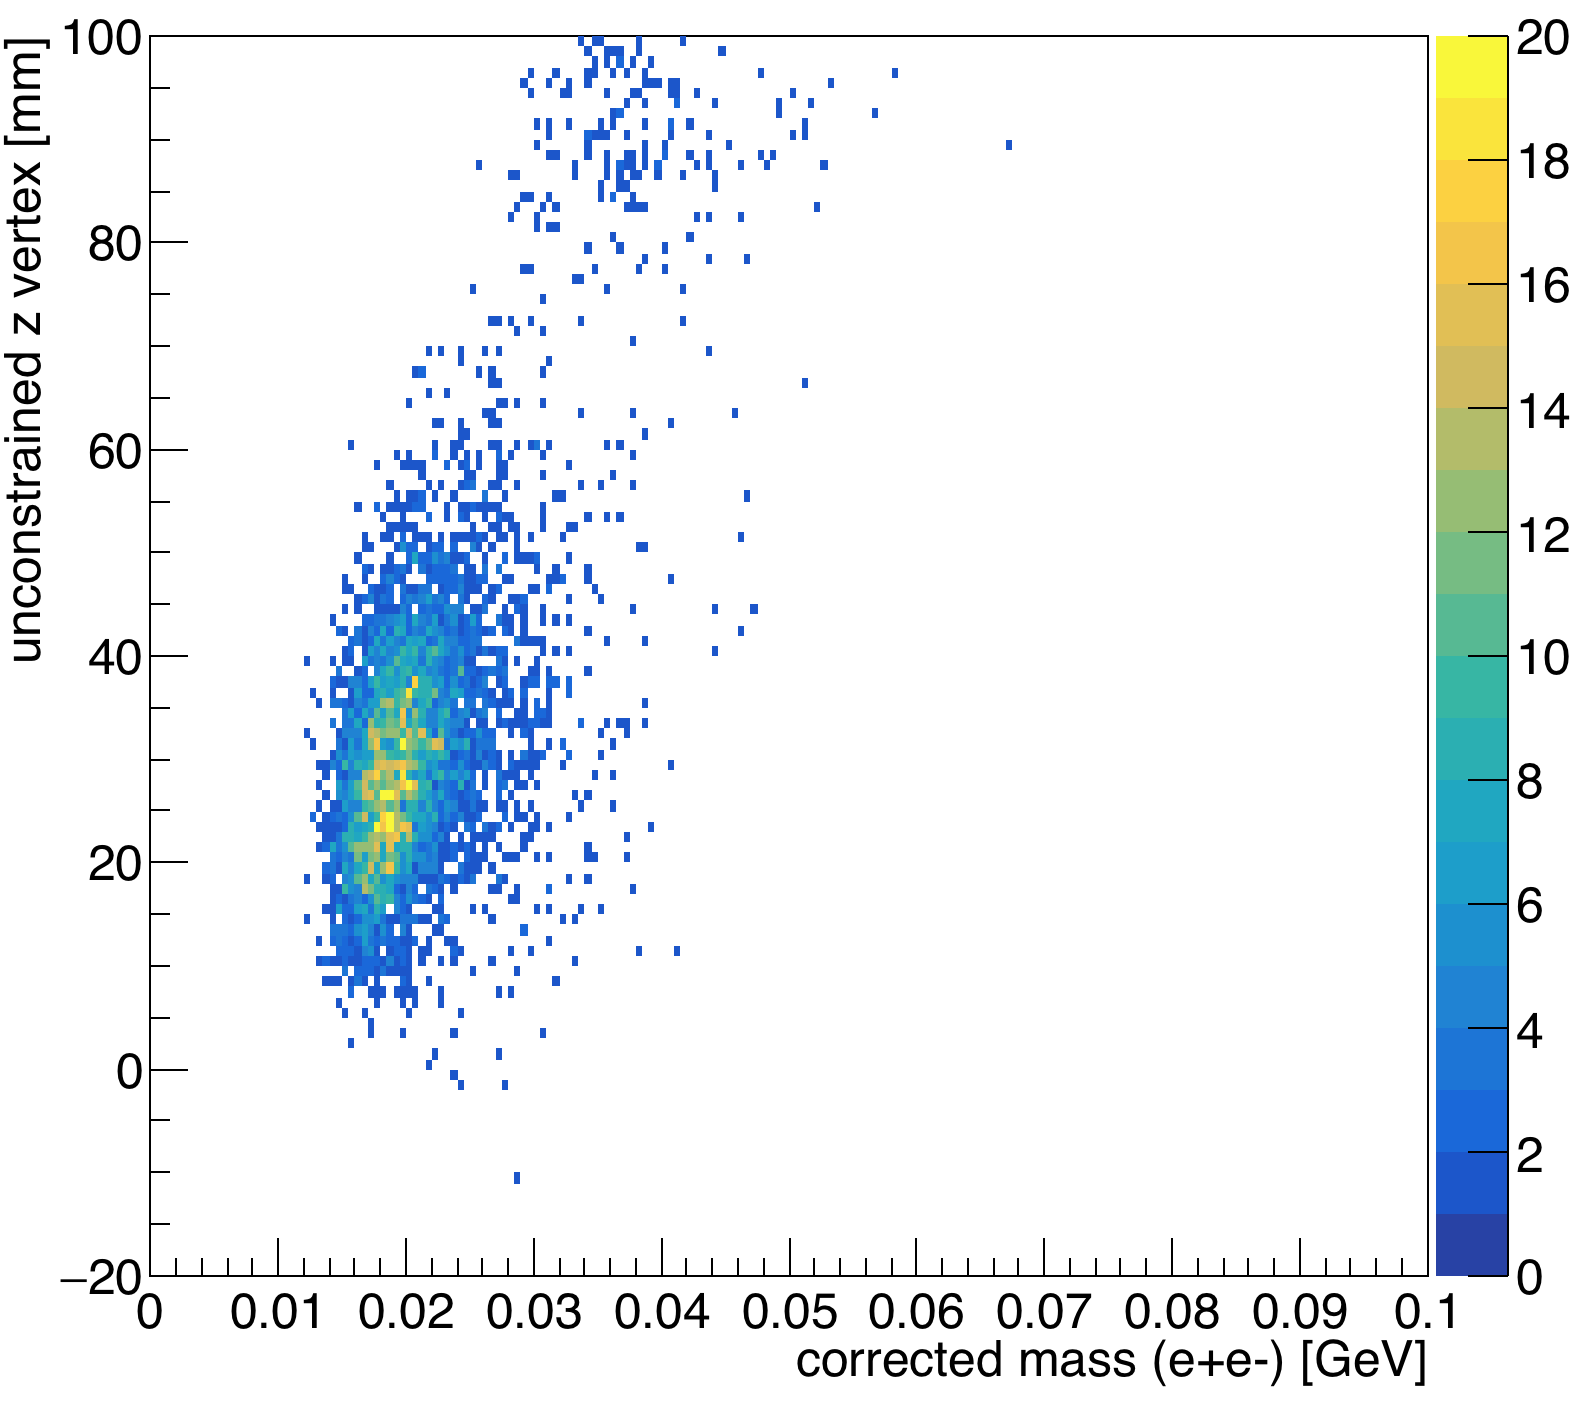
\includegraphics[width=\textwidth]{pics/appendix/zVm_L2L2.png}
 \end{minipage}
  \caption[$z$ vertex and mass distribution for the L2L2 data set with the SVT at $\pm0.5$~mm]{The unconstrained $z$ vertex position is shown as a function of the corrected mass
of the $e^+e^-$ pair where both tracks do not pass through the active region of Layer 1. The $zCut$ as measured for this data is shown in red
and corresponds to the full 100$\%$ data set where there is less than 0.5 background event beyond. The projected $zCut$ from the 10$\%$ of the data is shown in magenta. The relevant mass range used to measure $zCut$ is from 0.02--0.06~GeV based on measured statistics. The 10$\%$ sample for tuning cuts is shown on the left, and the full 100$\%$ of the data is shown on the right.}
  \label{fig:zvm_l2l2}
\end{figure}
The L2L2 data with the SVT at $\pm0.5$~mm from the beam is dominated by high $z$ backgrounds. This background appears to go all the way out to the first SVT layer. Due to this background alone, this data set cannot contribute to the projected reach. Ideally, there should be no events in this data set except for pure signal events. These events cannot be signal due to their uniform distribution over several masses. A $zCut$ should be able to be chosen for this data such that the reconstructed vertex efficiency can be optimized, but this is only true if the background events can be removed. \\
\indent The L2L2 data with the SVT slightly more open at $\pm1.5$~mm from the beam is shown in Figure~\ref{fig:zvm_l2l2_1p5}. The mass and $z$ vertex distribution for the L2L2 data taken with the SVT at 1.5~mm is shown in Figure~\ref{fig:zvm_l2l2_1p5}.
\begin{figure}[hbt]
\begin{minipage}{0.5\textwidth}
 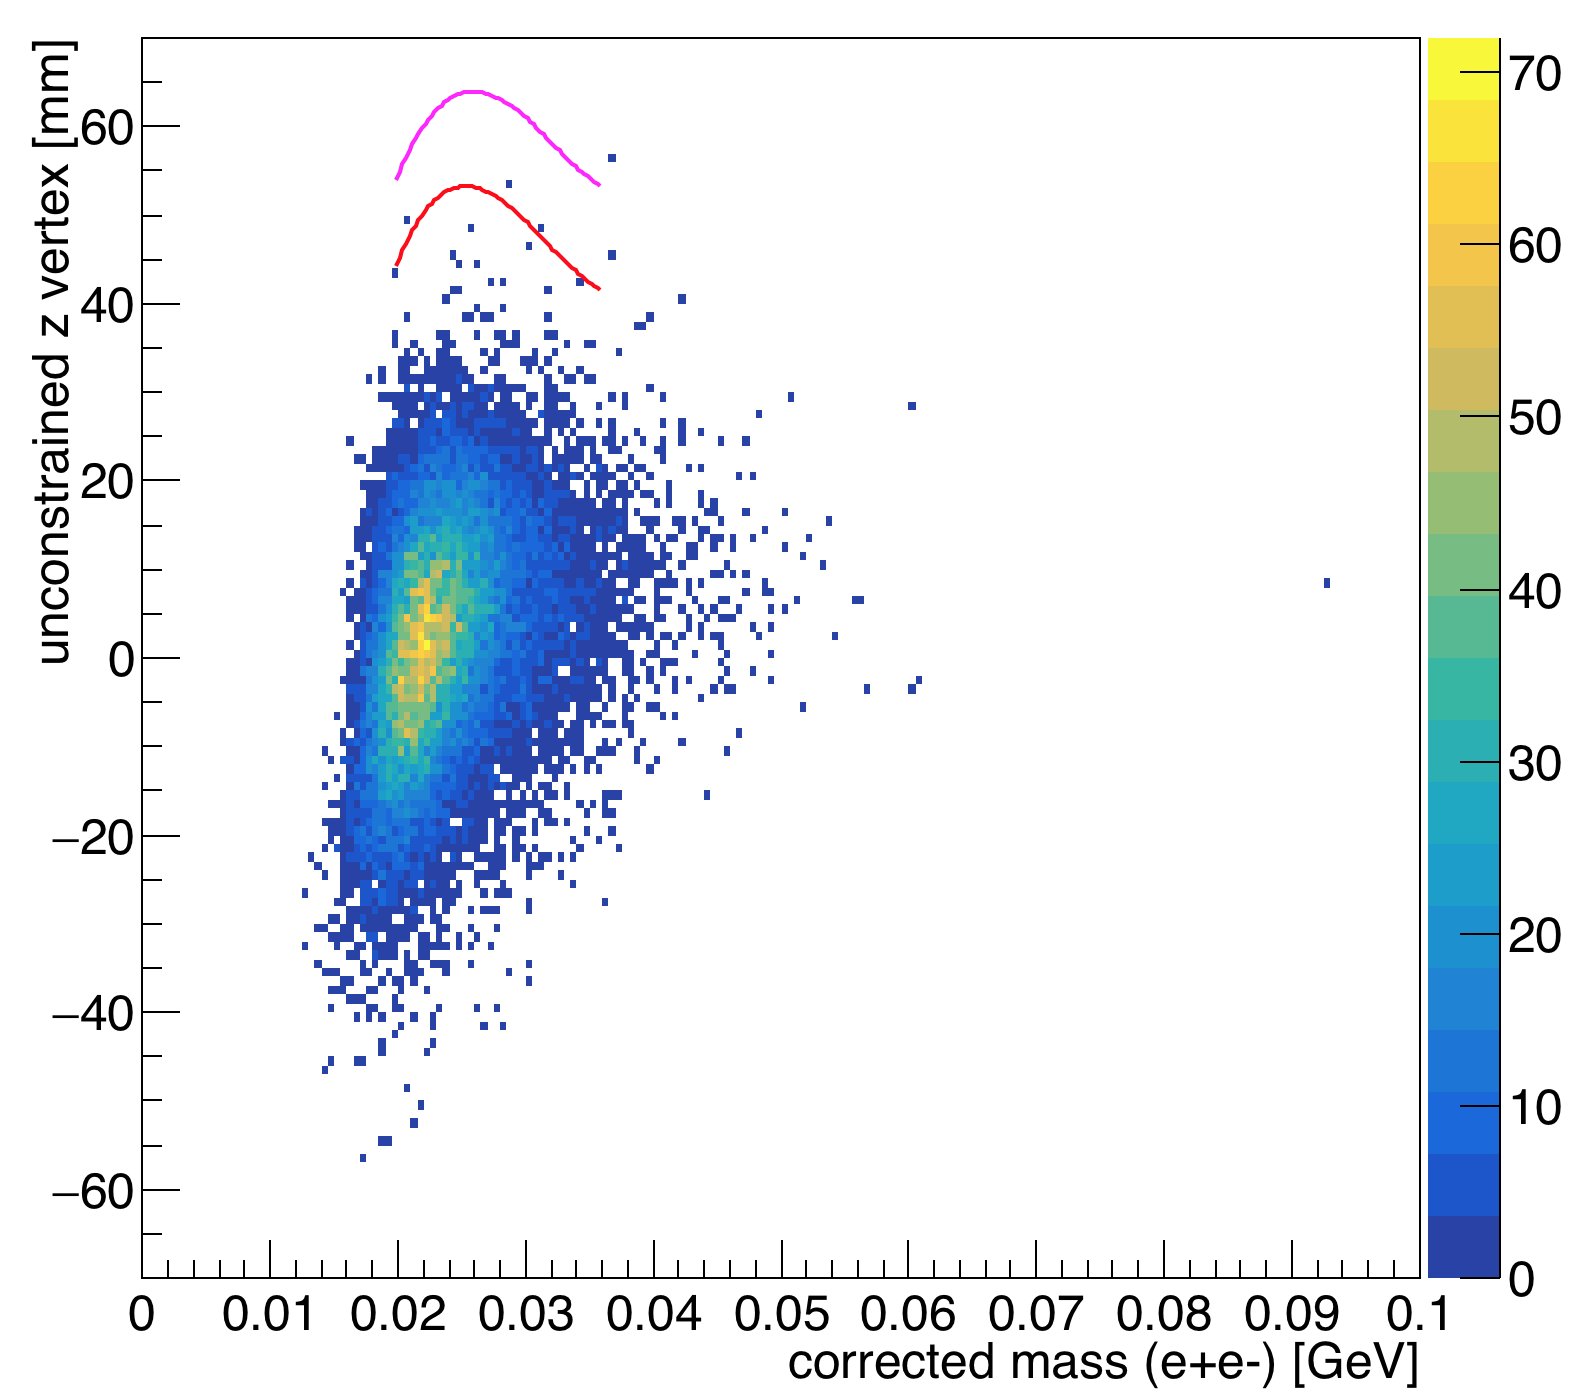
\includegraphics[width=\textwidth]{pics/appendix/zVm_L2L2_1p5_bl.png}
\end{minipage}\hfill\begin{minipage}{0.5\textwidth}
 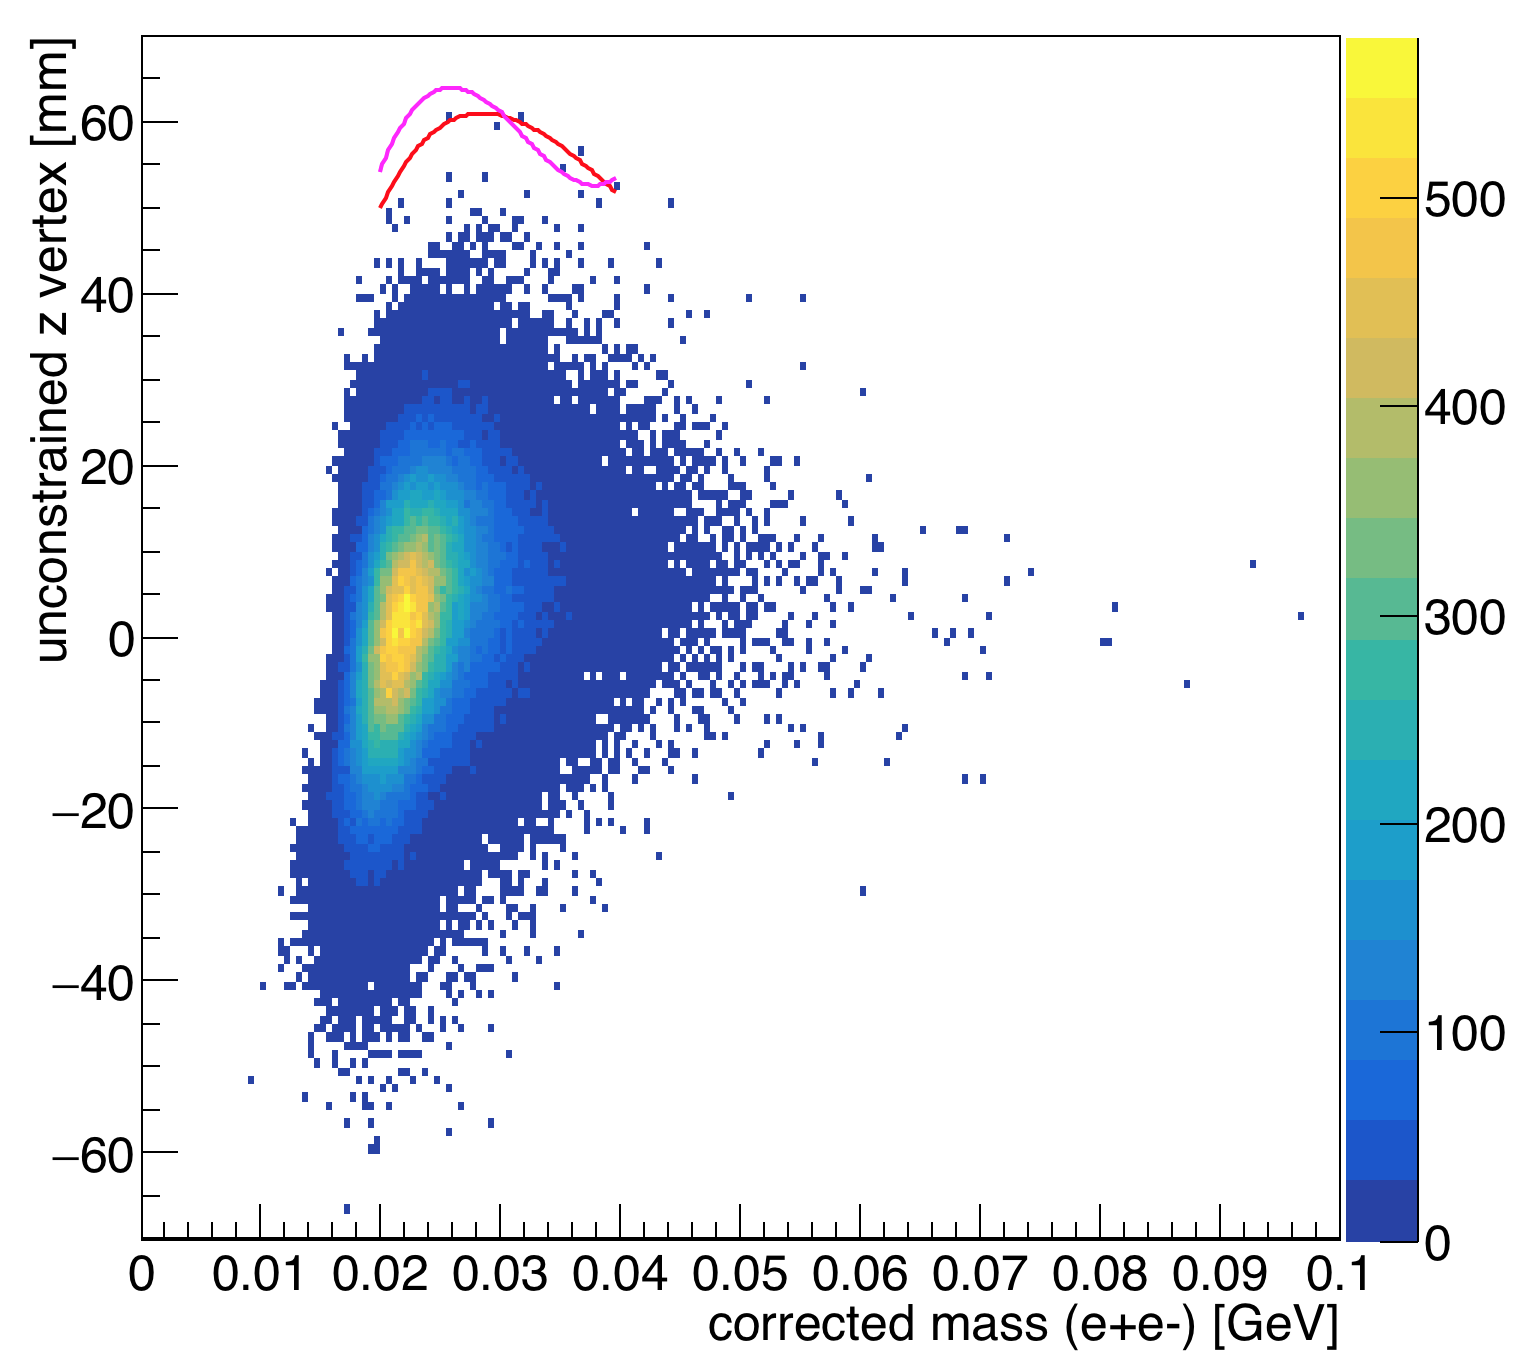
\includegraphics[width=\textwidth]{pics/appendix/zVm_L2L2_1p5_ub.png}
 \end{minipage}
  \caption[$z$ vertex and mass distribution for the L2L2 data set with the SVT at $\pm1.5$~mm]{The unconstrained $z$ vertex position is shown as a function of the corrected mass
of the $e^+e^-$ pair where both tracks do not pass through the active region of Layer 1. The $zCut$ as measured for this data is shown in red
and corresponds to the full 100$\%$ data set where there is less than 0.5 background event beyond. The projected $zCut$ from the 10$\%$ of the data is shown in magenta. The relevant mass range used to measure $zCut$ is from 0.02--0.04~GeV based on measured statistics. The 10$\%$ sample for tuning cuts is shown on the left, and the full 100$\%$ of the data is shown on the right.}
  \label{fig:zvm_l2l2_1p5}
\end{figure}
The L2L2 data at 1.5~mm has considerably fewer high $z$ background events than the data from 0.5~mm. While a $zCut$ for this data can be obtained, the statistics of the 1.5~mm data set are too low to obtain additional reach contributions. 